\section[Architetture non Von Neumann]{Architetture non Von Neumann}
\label{sec:pipeline}
\sectionframe{images/covers/cover_pipeline.png}{Architetture \protect\linebreak non Von Neumann}	 
 

\begin{frame}
	\frametitle{Aumentare le prestazioni delle CPU}

	\begin{block}{Aumentare le prestazioni delle CPU}
		Per potenziare le prestazioni delle CPU e dei sistemi di elaborazione, rimanendo ancorati ad una architettura di Von Neumann, sono state prese in considerazione diverse strategie:
		\begin{itemize}
			\item l'incremento della frequenza di clock
			\item l'ampliamento della dimensione della parola
			\item l'aumento dello spazio di indirizzamento
		\end{itemize}
		
		Tuttavia, tutte queste strategie hanno raggiunto un punto limite nell'evoluzione delle architetture, oltre il quale ulteriori miglioramenti delle prestazioni sono diventati sempre più difficili.\\~\\
		
		Di conseguenza, è emersa un'altra prospettiva di sviluppo attraverso l'approccio di \textbf{architetture non Von Neumann}.
	\end{block}

\end{frame}


\begin{frame}
	\frametitle{Aumentare le prestazioni delle CPU}

	\begin{figure}[!htbp]
		\centering
		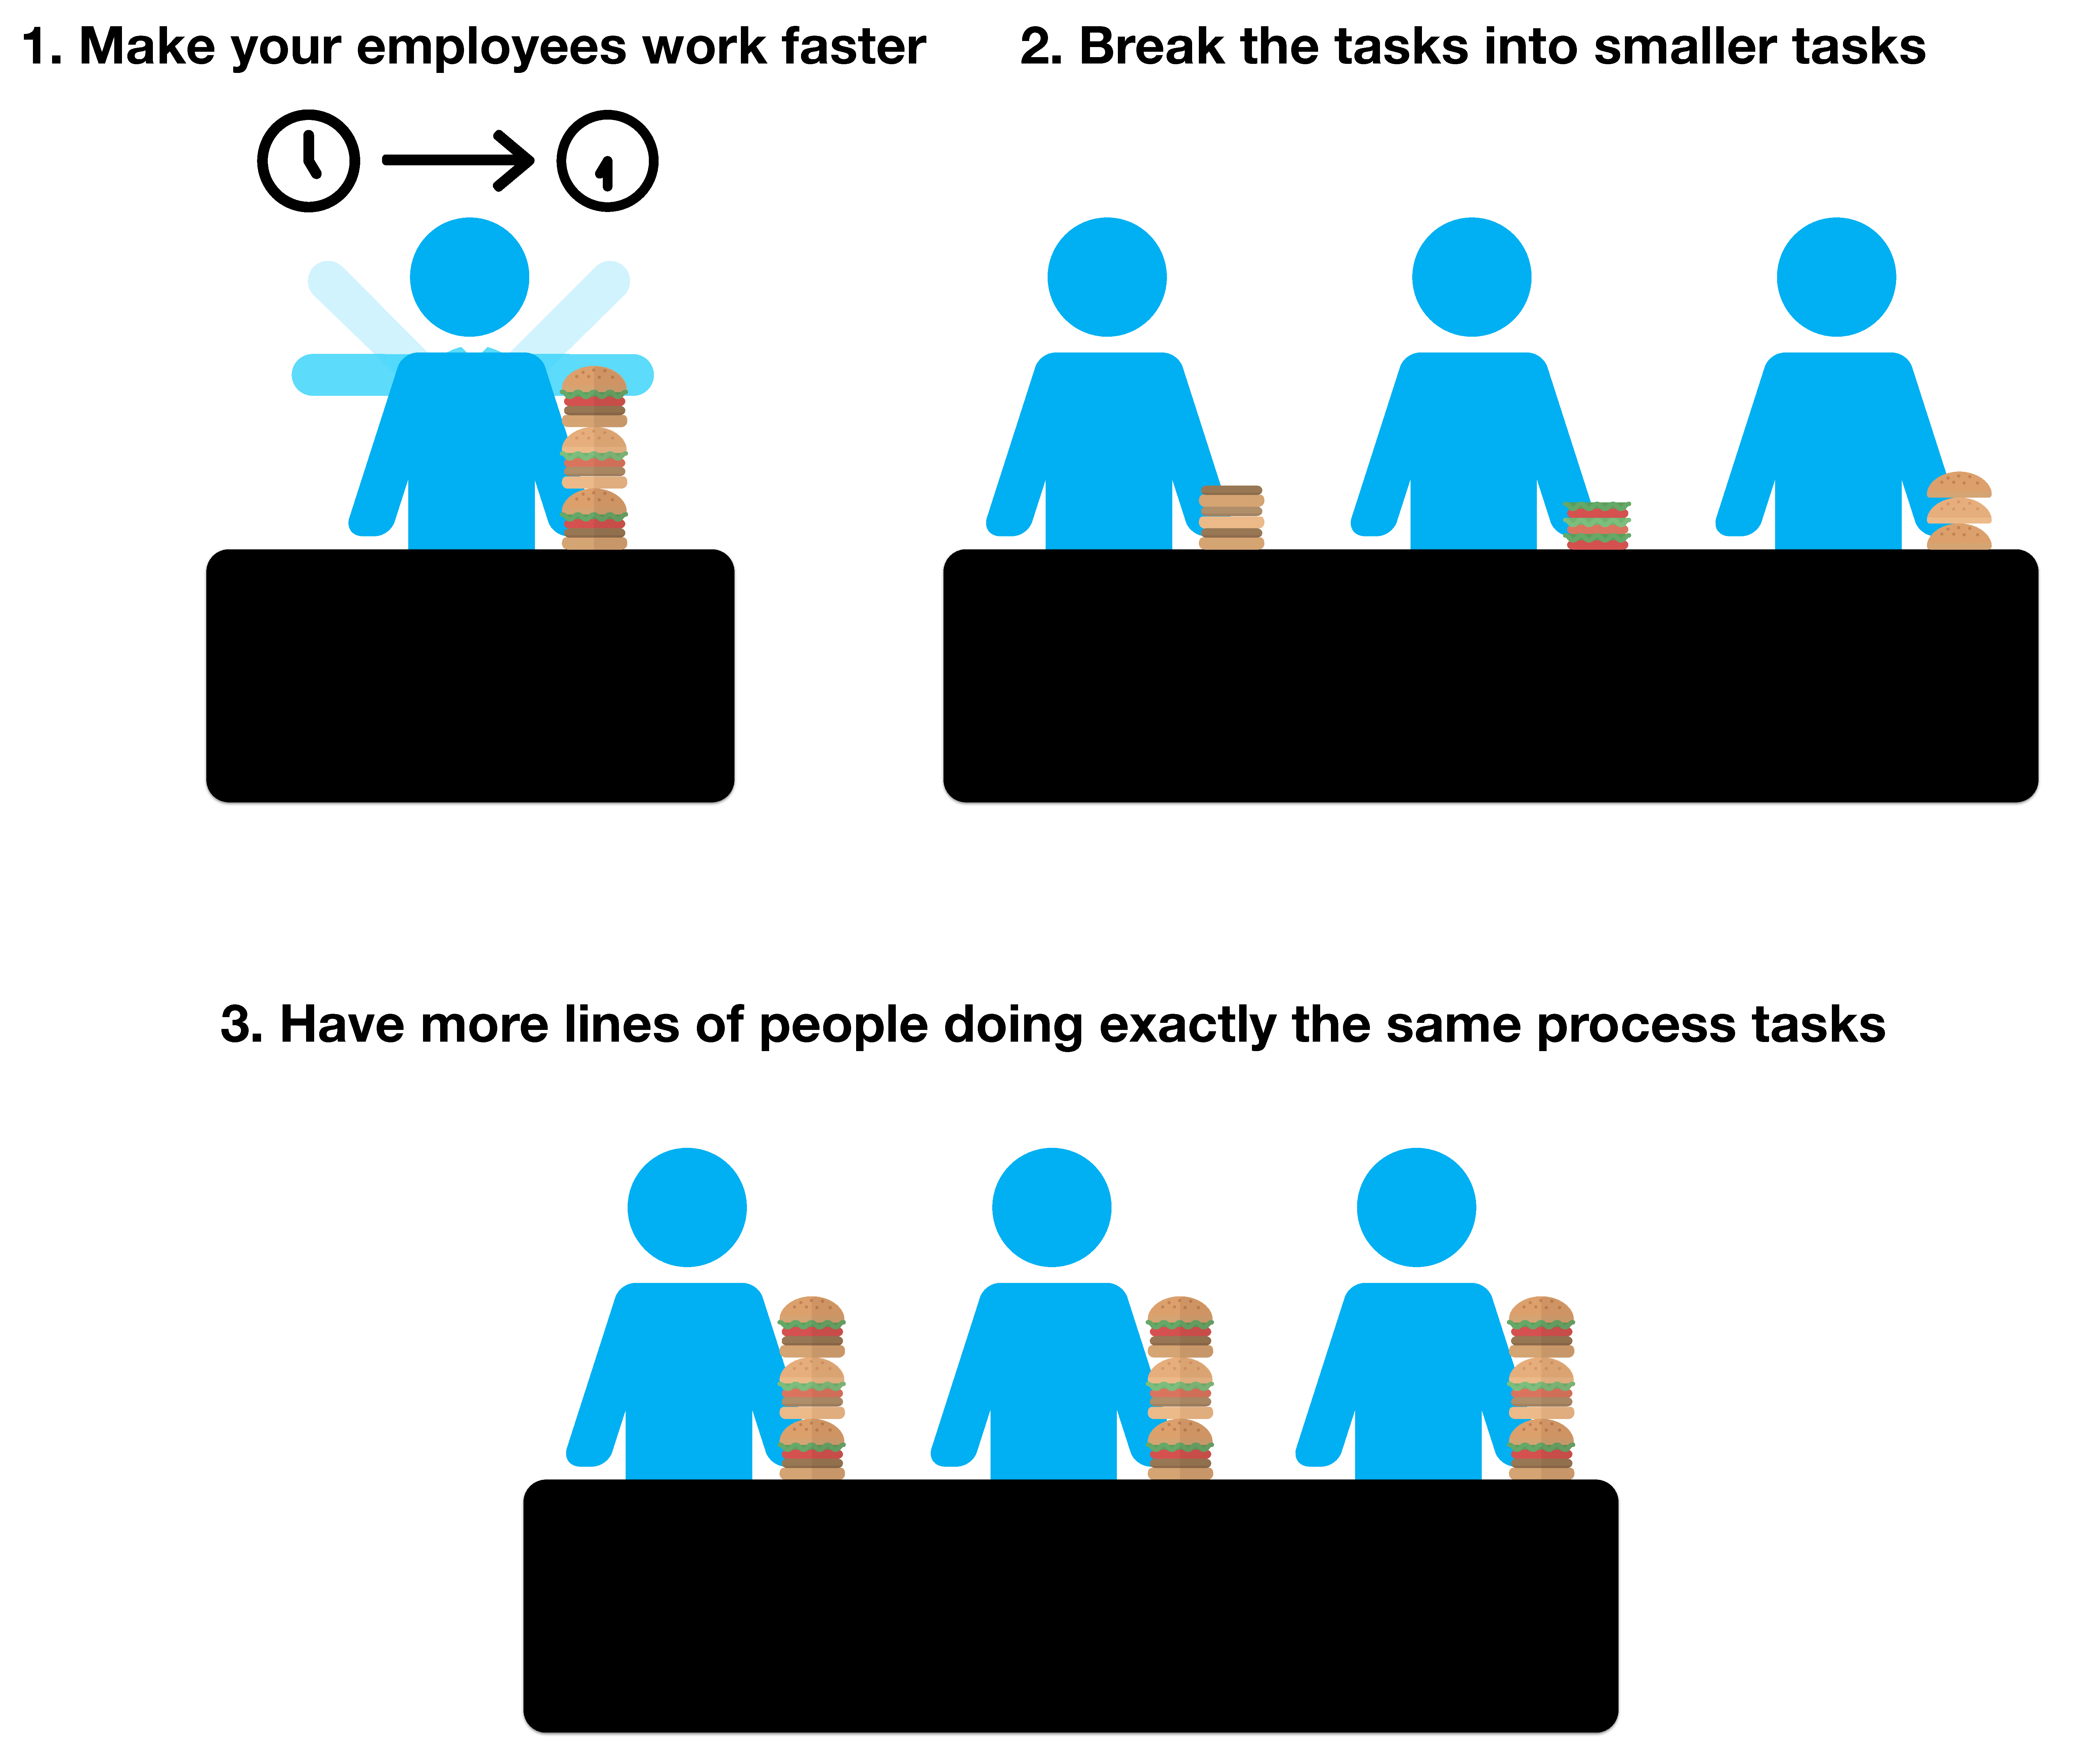
\includegraphics[width=0.73\linewidth]{images/7_pipeline/faster_cpu.pdf}
		%\caption{}
%		\label{}
	\end{figure}
\end{frame}


\begin{frame}
	\frametitle{Architetture non Von Neumann}

	\begin{block}{Architetture non Von Neumann}
		Elenchiamo alcune di questi possibili approcci:
		\begin{enumerate}
			\item Esecuzione fuori ordine
			\item Prefetch
			\item Speculative execution
			\item Pipeline
			\item Branch prediction
			\item Cache memory
			\item DMA (Direct Memory Access)
			\item Coprocessori
		\end{enumerate}
	\end{block}

\end{frame}


\subsection[Esecuzione fuori ordine]{Esecuzione fuori ordine}
\begin{frame}
	\frametitle{\textbullet{1} Esecuzione fuori ordine}

	%\begin{block}{Esecuzione fuori ordine}
		L'\textbf{esecuzione fuori ordine} è una tecnica avanzata utilizzata nelle CPU per migliorare l'efficienza nell'esecuzione delle istruzioni. Invece di eseguire le istruzioni nell'ordine in cui sono state ricevute, come accadeva nelle prime architetture, l'esecuzione fuori ordine permette alla CPU di eseguire istruzioni indipendenti in parallelo, sfruttando al massimo le risorse disponibili.\\~\\		
		Quando una CPU opera in modalità di esecuzione fuori ordine, può analizzare le istruzioni in entrata e identificare quelle che possono essere eseguite senza dipendenze da istruzioni precedenti. Queste istruzioni vengono inviate alle unità di esecuzione in parallelo, indipendentemente dall'ordine originale. Questo metodo \textbf{non sempre può essere impiegato}. Qualora due istruzioni consecutive siano dipendenti (ad esempio se la seconda istruzione usa il risultato ottenuto dalla prima istruzione) è necessario rispettare la sequenza operativa e le due istruzioni non potranno essere eseguite in parallelo.
	%\end{block}

\end{frame}


\begin{frame}
	\frametitle{\textbullet{1} Esecuzione fuori ordine}

	%\begin{block}{Esecuzione fuori ordine}
		L'esecuzione fuori ordine richiede hardware complesso, come buffer per riordinare i risultati in base all'ordine originale, unità di predizione delle dipendenze e logica per garantire l'integrità delle operazioni. Questa tecnica ha dimostrato di \textbf{migliorare notevolmente le prestazioni} delle CPU, consentendo loro di eseguire più istruzioni in modo parallelo e ottimizzato, pur mantenendo l'ordine corretto dei risultati in uscita.% \\~\\
		
		%
		
		\begin{figure}[!htbp]
			\centering 
			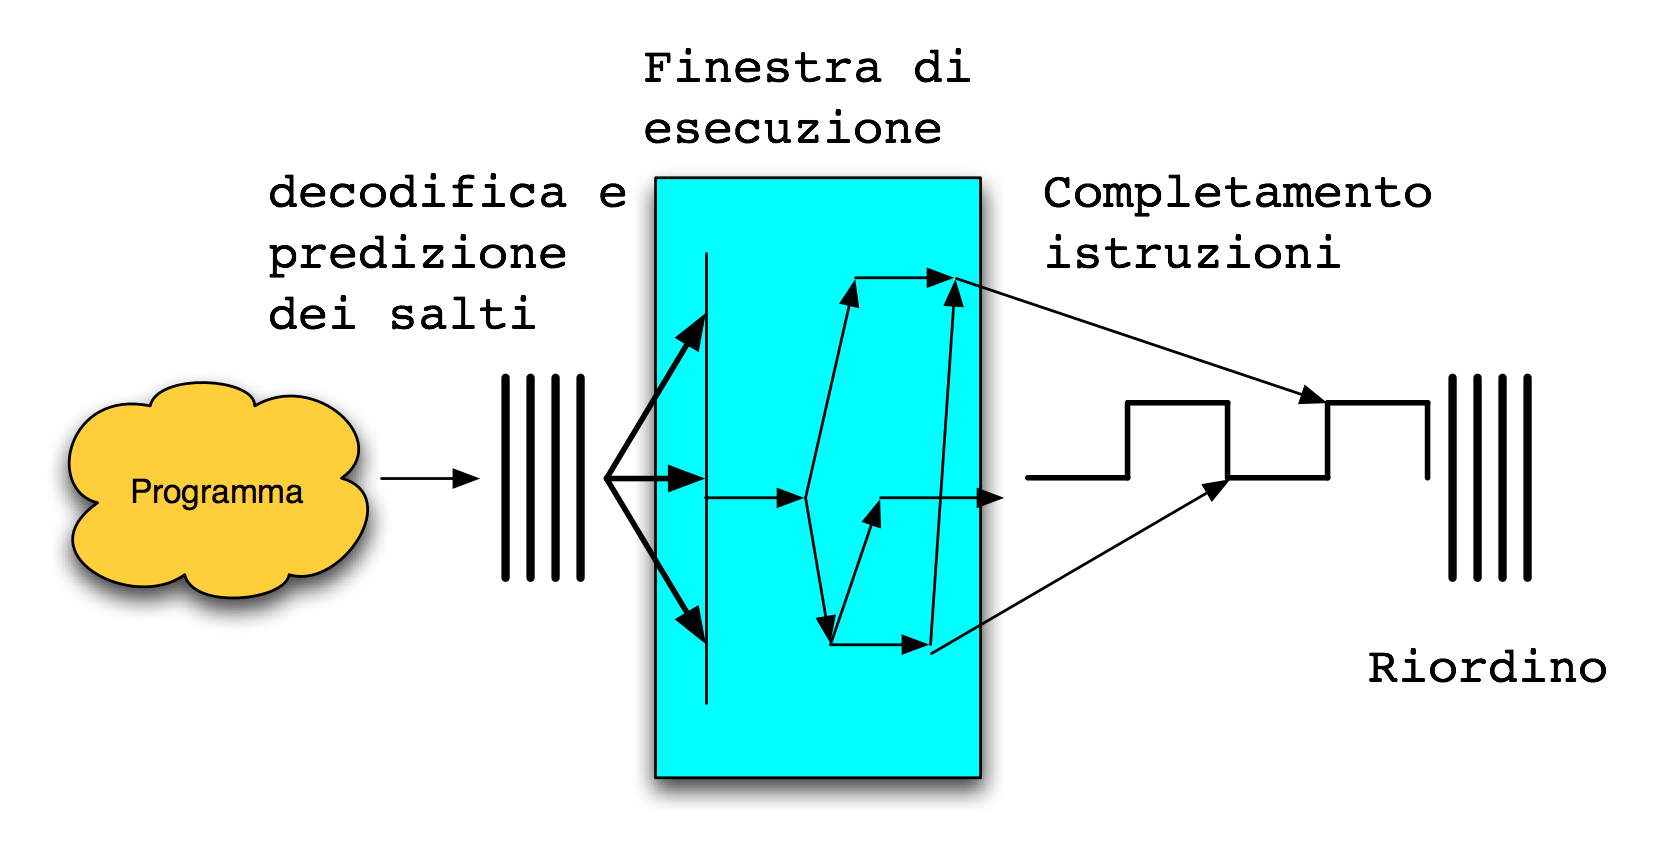
\includegraphics[width=0.7\linewidth]{images/7_pipeline/superscalar_processor.png}
			%\caption{}
			\label{fig:pipeline_superscalar_processor}
		\end{figure}
	%\end{block}

\end{frame}


\begin{frame}
	\frametitle{\textbullet{2} Prefetch}

	%\begin{block}{Esecuzione fuori ordine}
		Nel contesto delle CPU, il \textbf{prefetch} è una tecnica di ottimizzazione che coinvolge il caricamento anticipato dei dati dalla memoria principale alla cache prima che siano effettivamente richiesti dall'esecuzione del programma. L'obiettivo principale del prefetch è ridurre i tempi di attesa e migliorare l'efficienza complessiva del sistema.\\~\\
		Il prefetch cerca di \textbf{prevedere quali dati saranno richiesti} successivamente e anticipa questo processo, caricando questi dati nella cache in modo che siano pronti per essere utilizzati quando verranno effettivamente richiesti. Questo può ridurre i ritardi dovuti all'accesso alla memoria, poiché i \textbf{dati richiesti sono già disponibili nella cache}, che è molto più veloce della memoria principale.
	%\end{block}

\end{frame}


\begin{frame}
	\frametitle{\textbullet{3} Speculative execution}

	%\begin{block}{Esecuzione fuori ordine}
		La \textbf{speculative execution} (esecuzione speculativa) è una tecnica avanzata utilizzata nelle CPU per ottimizzare le prestazioni \textbf{eseguendo istruzioni} in \textbf{anticipo sulla base di previsioni}. Quando la CPU incontra un ramo condizionale (come un'istruzione di salto o un'istruzione condizionale), anziché attendere il risultato della condizione, la CPU esegue istruzioni speculativamente, seguendo la previsione più probabile.\\~\\
		\textbf{L'obiettivo della speculative execution è mitigare i ritardi causati dalle ramificazioni condizionali}. Se la previsione è corretta, l'esecuzione speculativa ha permesso alla CPU di eseguire istruzioni extra durante l'attesa della risposta condizionale. Tuttavia, se la previsione è errata, la CPU scarta semplicemente i risultati dell'esecuzione speculativa e riprende l'esecuzione dal punto corretto.\\
		Questa tecnica comporta l'utilizzo di unità di predizione dai branch per stimare quale sarà l'esito di una decisione condizionale.
	%\end{block}

\end{frame}


\begin{frame}
	\frametitle{\textbullet{4} Pipeline}

	%\begin{block}{Esecuzione fuori ordine}
		La \textbf{pipeline} nei PC e nell'architettura dei processori si riferisce a una tecnica di progettazione che suddivide l'esecuzione di istruzioni in diverse \textbf{fasi sequenziali}. Ogni fase rappresenta una parte del processo di esecuzione dell'istruzione, come il prelievo dell'istruzione dalla memoria, la decodifica dell'istruzione, l'esecuzione dell'istruzione e la scrittura dei risultati (rispettivamente fetch, decode, execute e write-back).\\~\\
		Questa suddivisione consente al processore di eseguire istruzioni in modo più efficiente e parallelo. Mentre un'istruzione è in fase di decodifica, il processore può iniziare a elaborare la successiva istruzione. Questo approccio riduce il tempo in cui il processore deve attendere che un'istruzione si completi prima di iniziare la successiva, aumentando così l'utilizzo delle risorse del processore.
	%\end{block}

\end{frame}


\begin{frame}
	\frametitle{\textbullet{4} Pipeline: laundry analogy}

	%\begin{block}{Esecuzione fuori ordine}
				
		\begin{figure}[!htbp]
			\centering 
			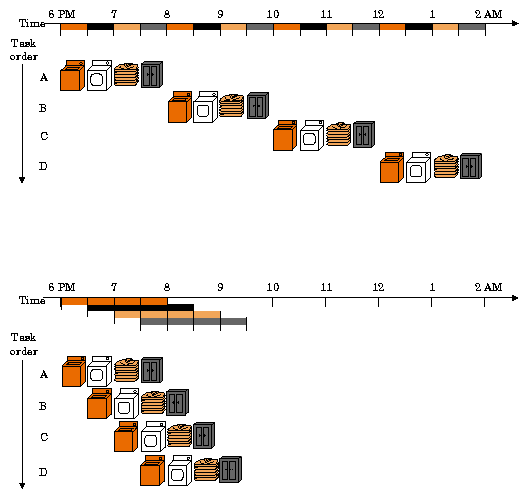
\includegraphics[width=0.5\linewidth]{images/7_pipeline/laundry_analogy.png}
			\caption{\textbf{Washer} takes 30 minutes, \textbf{Dryer} takes 30 minutes, \textbf{Folder} takes 30 minutes and \textbf{Stasher} takes 30 minutes: without pipeline to execute A, B, C, D tasks you would need 8 hours, with pipeline just 3.5 hours.}
			%\label{}
		\end{figure}
	%\end{block}

\end{frame}


% https://en.wikibooks.org/wiki/Microprocessor_Design/Pipelined_Processors
% https://en.wikipedia.org/wiki/Instruction_pipelining

\begin{frame}
	\frametitle{\textbullet{4} Pipeline}

	%\begin{block}{Esecuzione fuori ordine}
		Il numero di fasi varia in base all'architettura della macchina.\\
		La classica pipeline RISC comprende:
		\begin{itemize}
			\item Instruction fetch
			\item Instruction decode and register fetch
			\item Execute
			\item Memory access
			\item Register write back
		\end{itemize}
		
		Più una pipeline è \textit{profonda} (con un numero maggiore di fasi), più una specifica fase può essere implementata con una circuiteria più semplice. Tali pipeline possono essere chiamate \textit{superpipeline}.\\
		Si dice che un processore è \textbf{fully pipelined} se è in grado di recuperare un'istruzione ad ogni ciclo. Pertanto, se alcune istruzioni o condizioni richiedono ritardi che inibiscono il recupero di nuove istruzioni, il processore non è \textit{fully pipelined}.
	%\end{block}

\end{frame}


\begin{frame}
	\frametitle{\textbullet{4} Pipeline}

	%\begin{block}{Esecuzione fuori ordine}
		Le fasi della classica pipeline RISC:
		\begin{itemize}
			\item \textbf{Instruction fetch (IF)}:\\ lettura dell'istruzione dalla memoria
			\item \textbf{Instruction decode and register fetch (ID)}:\\ decodifica dell'istruzione e lettura degli operandi da registri
			\item \textbf{Execute (EX)}:\\ esecuzione dell’istruzione
			\item \textbf{Memory access (MEM)}:\\ attivazione della memoria
			\item \textbf{Register write back (WB)}:\\ scrittura del risultato nel registro opportuno
		\end{itemize}
		
		\begin{figure}[!htbp]
			\centering 
			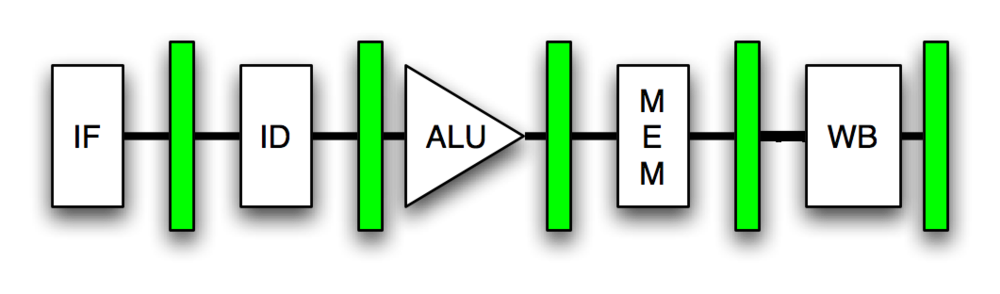
\includegraphics[width=0.63\linewidth]{images/7_pipeline/pipeline_base.png}
			%\caption{}
			\label{fig:pipeline_pipeline_base}
		\end{figure}
		
	%\end{block}

\end{frame}


\begin{frame}
	\frametitle{\textbullet{4} Pipeline}

	%\begin{block}{Esecuzione fuori ordine}
		\begin{figure}[!htbp]
			\centering 
			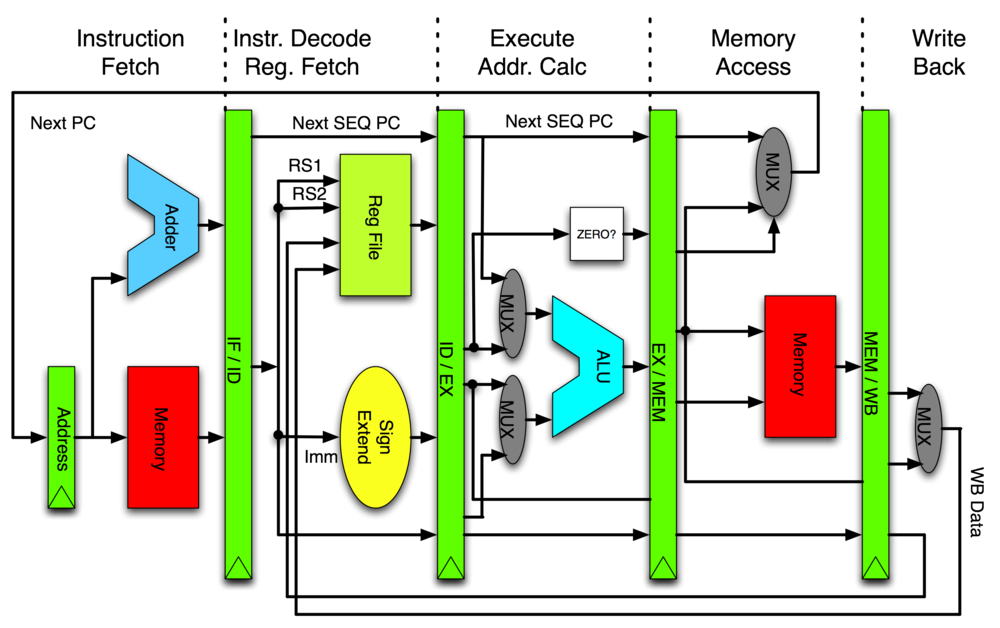
\includegraphics[width=0.82\linewidth]{images/7_pipeline/pipeline_mips_structure.png}
			\caption{Una architettura MIPS in 5 fasi}
			% (Microprocessor without Interlocked Pipelined Stages)
			\label{fig:pipeline_mips_structure}
		\end{figure}
	%\end{block}

\end{frame}


\begin{frame}
	\frametitle{\textbullet{4} Pipeline}

	%\begin{block}{Esecuzione fuori ordine}
		\begin{figure}[!htbp]
			\centering 
			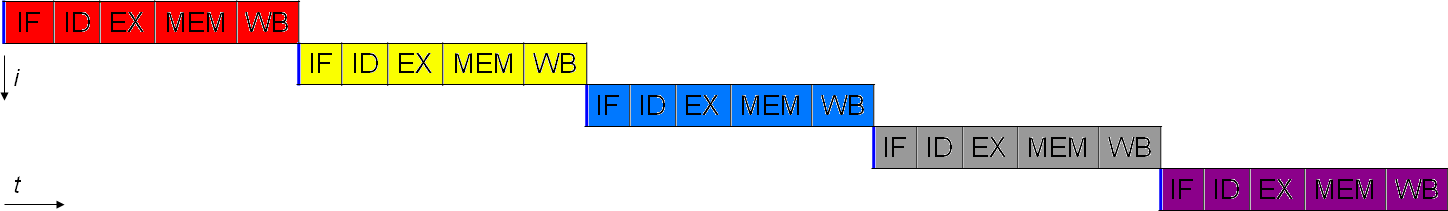
\includegraphics[width=1.0\linewidth]{images/7_pipeline/pipeline_no.png}
			\caption{Se eseguissi 5 istruzioni senza sfruttare la pipeline in ogni istante di tempo sarebbe presente una sola istruzione alla volta all'interno della pipeline}
%			\label{}
		\end{figure}
	%\end{block}

\end{frame}


\begin{frame}
	\frametitle{\textbullet{4} Pipeline}

%	\begin{block}{Esecuzione fuori ordine}
%		\begin{columns}
%			\column{0.5\linewidth}
%			\begin{figure}[!htbp]
%				\centering 
%				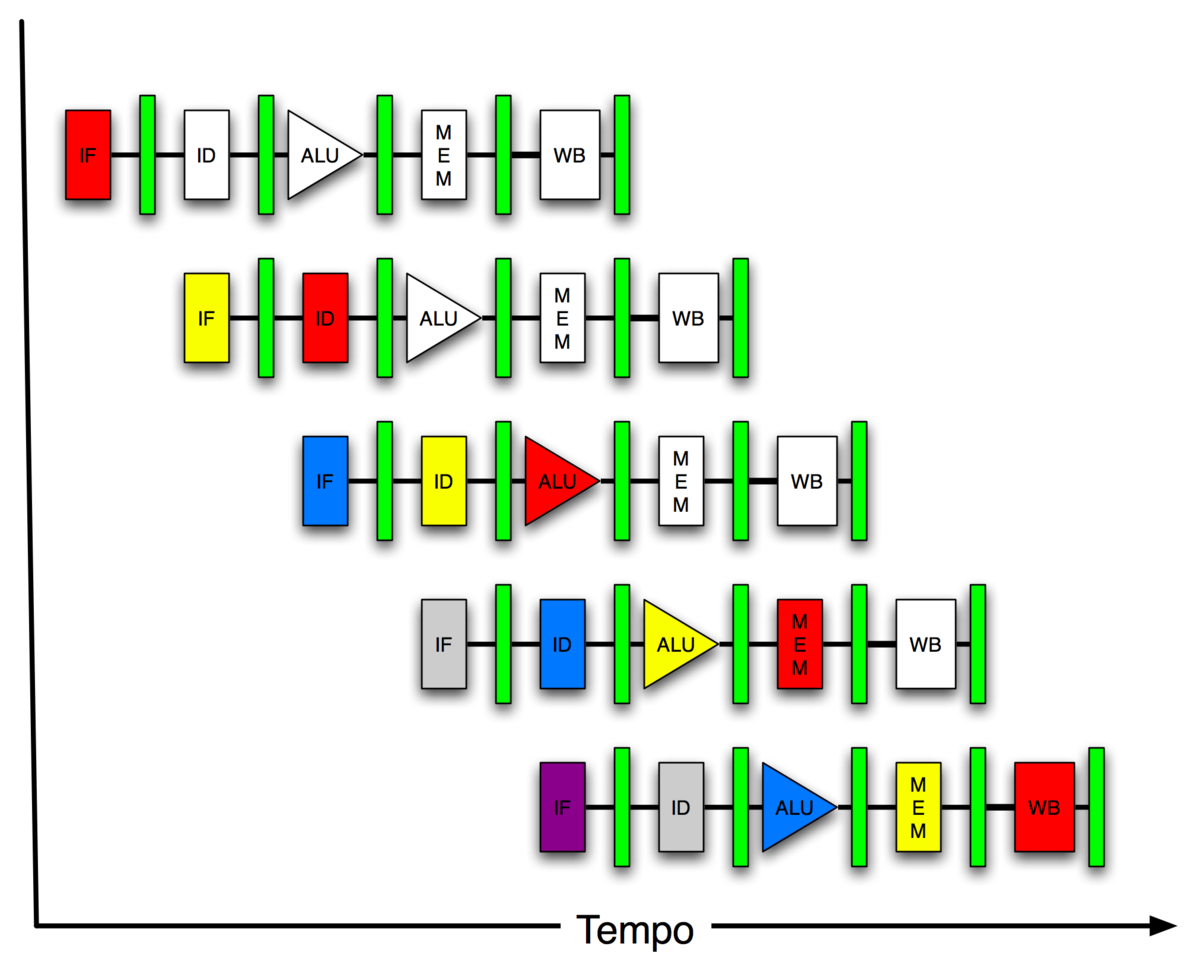
\includegraphics[width=1.0\linewidth]{images/7_pipeline/pipeline_in_time.png}
%				\caption{Se abbiamo 5 istruzioni, possiamo mostrarle nella nostra pipeline utilizzando colori diversi. Nel diagramma seguente, il bianco corrisponde a un NOP e i diversi colori corrispondono alle istruzioni nella pipeline. In ogni fase, le istruzioni avanzano attraverso la pipeline.}
%				\label{fig:pipeline_pipeline_in_time}
%			\end{figure}
%				
%			\column{0.5\linewidth}
%			\begin{figure}[!htbp]
%				\centering 
%				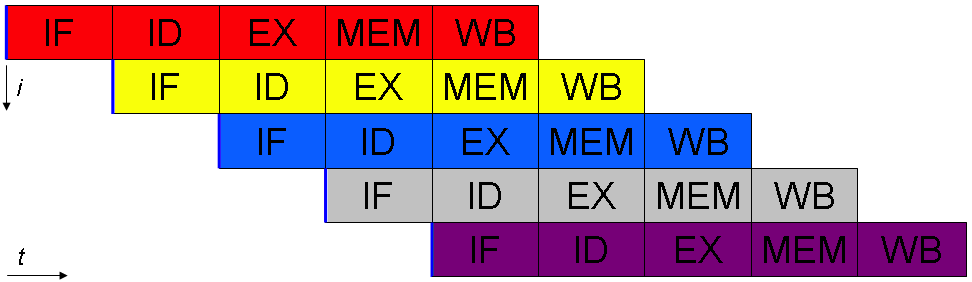
\includegraphics[width=1.0\linewidth]{images/7_pipeline/pipeline_five_stages.png}
%	%			\caption{}
%	%			\label{}
%			\end{figure}
%		\end{columns}
		
		
		\begin{figure}[htbp]
		    \centering
		    \begin{minipage}{0.49\textwidth}
		        \centering
		        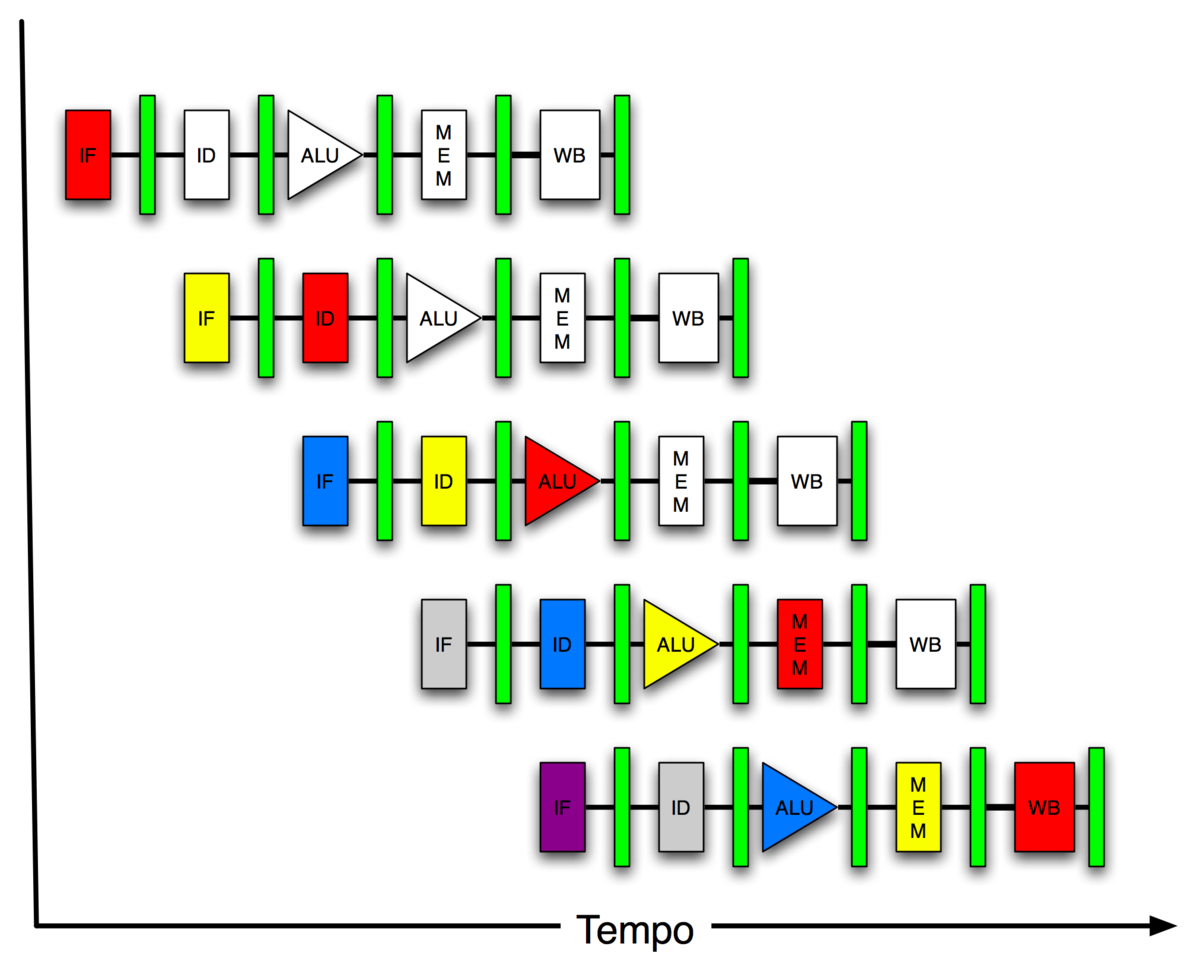
\includegraphics[width=1.0\linewidth]{images/7_pipeline/pipeline_in_time.png}
		    \end{minipage}
		    \hfill
		    \begin{minipage}{0.49\textwidth}
		        \centering 
				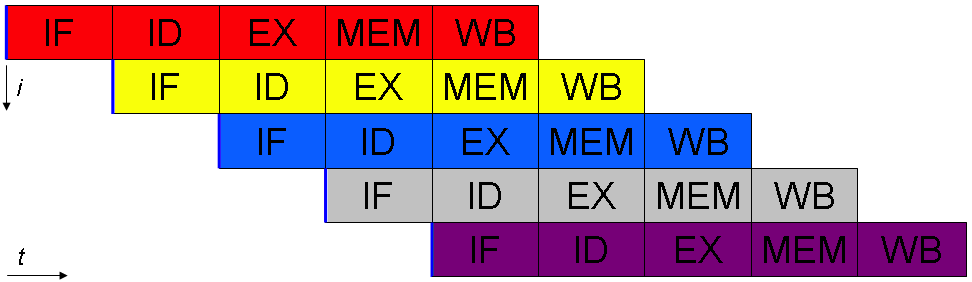
\includegraphics[width=1.0\linewidth]{images/7_pipeline/pipeline_five_stages.png}
		    \end{minipage}
		    \caption{Se abbiamo 5 istruzioni, possiamo mostrarle nella nostra pipeline utilizzando colori diversi. Nel diagramma seguente, il bianco corrisponde a un NOP e i diversi colori corrispondono alle istruzioni nella pipeline. In ogni fase, le istruzioni avanzano attraverso la pipeline.}
		    \label{fig:pipeline_pipeline_in_time}
		\end{figure}
		
	%\end{block}

\end{frame}



\begin{frame}
	\frametitle{\textbullet{4} Pipeline}

	%\begin{block}{Esecuzione fuori ordine}
		Tuttavia, la pipeline può incontrare situazioni in cui le istruzioni successive dipendono dai risultati di quelle precedenti.
		
	%\end{block}

\end{frame}






\subsection[Prefetch]{Prefetch}
\subsection[Speculative execution]{Speculative execution}
\subsection[Pipeline]{Pipeline}
\subsection[Branch prediction]{Branch prediction}
\subsection[Cache memory]{Cache memory}
\subsection[DMA (Direct Memory Access)]{DMA (Direct Memory Access)}
\subsection[Coprocessori]{Coprocessori}





%\subsection[Central Processing Unit]{Central Processing Unit}
%\begin{frame}
%	\frametitle{Central Processing Unit}
%	
%%	\begin{block}{Central Processing Unit}
%		Una CPU, \textbf{central processing unit} (unità centrale di elaborazione o processore centrale), indica un'unità o sottosistema logico e fisico che sovraintende alle \textbf{funzionalità logiche di elaborazione} principali di un computer.
%		La CPU è un'elaborata combinazione di transistor che può essere definita \textit{circuito integrato}.\\~\\
%		\pause
%		All'interno della CPU individuiamo tre elementi fondamentali:
%		\begin{itemize}
%			\item \textbf{la CU}, \textit{Control Unit} (l’unità di controllo):\\
%			coordina l'esecuzione delle operazioni da parte del processore;
%			\item \textbf{la ALU}, \textit{Arithmetic-Logic Unit} (l’Unità Aritmetico-Logica):\\
%			si occupa di eseguire le operazioni aritmetico-logiche;
%			\item \textbf{i registri di memoria}:\\
%			diverse \textit{celle di memoria} dedicate a scopi specifici che vengono utilizzati per il controllo dell'esecuzione di un programma.
%		\end{itemize}
%%	\end{block}
%	
%\end{frame}


